\cotefile{149}
\scanpage{28}
\deleted{élémentaire d'Artin \inserted{anabélienne} -- donc son $\pi_1$ \deleted{est} \unsure{a|-} un centre trivial. Ceci posé}

\uline{Corollaire 2} La conclusion \inserted{$f=g$} du corollaire précédent \deleted{b)}, \deleted{\unsure{sera|est}} \inserted{est} valable si \deleted{au lieu de supposer $f$ ou $g$ \unsure{dominants|dominant},} on suppose \inserted{que $k$ est de car. $0$, $X$ \uline{normal}, et} \deleted{enfin:} on est dans l'une des hyp. suivantes

c) l'image de $\pi_1(f)$ est un sous-groupe ouvert de $\pi_1(Y)$, \inserted{$Y$ est une variété élémentaire d'Artin anabélienne}

d) l'image \inserted{de $\pi_1(X)$} par $\pi_1(f)$ \deleted{de tout sous-groupe ouvert de $\pi_1(X)$} a un centralisateur dans $\pi_1(Y)$ réduit à $(1)$ ; \deleted{\unsure{$X$ normal|$X$ admet}} \deleted{\unsure{on|un}} \inserted{et $Y$ se plonge dans un groupe alg. extension d'une VA par un tore}

\deleted{e) Le centre de $\pi_1(X)$, et le centralisateur de son image dans $\pi_1(Y)$, sont réduits à $1$.}
\margin{\fbox{\parbox{0.26\textwidth}{\deleted{\unsure{Remarquons} si $Y$ est \unsure{simple}, \unsure{centre} \unsure{est non|$\ne1$} \unsure{réduit} \unsure{à un point},}}}}

Comme le centralisateur d'un sous-groupe ouvert de $\pi_1(Y)$ ($\pi_1(Y)$ étant ext. successive de groupes profinis \uline{libres} anabéliens) est réduit à $(1)$, comme on a vu${}^*$ plus haut, le cas c) est un \deleted{\unsure{des variétés|de même} $X$ \unsure{aurait}} cas particulier de d); \deleted{D'autre part, d) se ramène à e), en remplaçant $X$ par un ouvert d'Artin} -- mais (dans le cas d), quitte à remplacer $X$ par un ouvert d'Artin (la normalité assurant que $\pi_1(U)\unsure{\longrightarrow|-}\pi_1(X)$ \unsure{surj.|surj}\unsure{)),|))|),}

\margin{${}^*$ il faut quand $\overline m$ travailler! pour le cas du $\pi_1$ d'une courbe complète de genre $g\geq2$ -- et vérifier que son $\pi_1$ est à centre trivial et qu'il n'a pas \unsure{d'éléments|d'élts} d'ordre fini! Sinon, se borner dans le cor. \unsure{au|aux} cas \unsure{de|des} fibres successives non complètes.}
\margin{27}

\scanpage{29}
\deleted{OPS de plus que $\pi_1(X)$ \illegible{1} un centre trivial. \unsure{En} car. $p>0$, notons qu'il \unsure{suffit} de \unsure{travailler} \unsure{avec} les groupes \unsure{fondamentaux} \unsure{premiers} à $p$ -- et $\unsure{\overline m|=}$ sur les \unsure{localisations|localisés} en $\ell\ne p$ des \unsure{groupes} \unsure{fondamentaux}.}
\mspage{14}

La situation $X,Y,f,g$ provient, par extension du corps de base, d'une situation analogue sur un corps $K$ \inserted{extension} de type fini \deleted{de} $\mathbb Q$. \deleted{\unsure{Choisissons} une} \inserted{Soit $\overline K$ la} clôture algébrique \deleted{$\unsure{\overline K|\overline Q}$} de $K$ dans $k$, \deleted{\unsure{des $k$ l'|des $f_k\,\ell$}} \inserted{et $\overline X,\overline Y,\overline f,\overline g$ \deleted{\unsure{sur|se}}} déduite de \inserted{$X,Y$,} $f,g$ par extension du corps de base de $K$ à $\overline K$. On a donc $\pi_1(\overline f)\ne\pi_1(\overline g)$ satisfaisant la condition d) avec de plus $\pi_1(\overline X)$ a centre trivial.

Mais ces \unsure{hypothèses|hyp. mises} impliquent que les extensions $\mathcal E_{\inserted{X/K}}\deleted{(X)}\inserted{=\pi_1(X)}$, $\mathcal E_{\inserted{Y/K}}\deleted{(Y)}\inserted{=\pi_1(Y)}$ de $\mathcal E_{\overline K/K}$ par $\pi_1(\overline X)$, resp. $\pi_1(\overline Y)$, ainsi que les hom $\pi_1(f)$, $\pi_1(g)$ induits, sont réconstruits à partir de \inserted{$\pi_1(\overline X)$, $\pi_1(\overline Y)$, de} $\pi_1(\overline f)$, $\pi_1(\overline g)$ et de l'action extérieure de $\mathcal E_{\overline K/K}$ sur ces groupes. On va montrer maintenant le
\margin{28}

\scanpage{30}
\uline{Corollaire 3} Soient \deleted{$f,g$} $X,Y$ deux schémas de type fini sur un corps $K$ ext. de type fini de $\mathbb Q$, \deleted{\unsure{tels|tel}} \inserted{on suppose} que $Y$ se plonge dans \unsure{une|un} \deleted{\unsure{VA|V.A.}} extension d'une V.A. par un tore, $X$ réduit, \deleted{\unsure{d'où}} \inserted{$X,Y$ géom. $0$-connexes. Soit} $\overline K$ une clôture algébrique de $K$, d'où des extensions ``extérieures'' $\mathcal E_{X/K}$, \inserted{$\mathcal E_{Y/K}$,} de $\mathcal E_{\overline K/K}=\operatorname{Gal}(\overline K/K)$ par $\pi_1(\overline X)$, $\pi_1(\overline Y)$, et pour $\unsure{\forall|A}$ morphisme $f:X-Y$, un morphisme $\pi_1(f)$ de $\mathcal E_{X/K}$ \inserted{\deleted{\unsure{par|dans}} dans $\mathcal E_{Y/K}$.}

Soient $f,g:X=Y$ tels que $\pi_1(f)=\pi_1(g)$ extérieurement -- i.e. $\pi_1(f)$ et $\pi_1(g)$ soient conjugués par un élément de $\pi_1(Y)$ -- alors $f=g$.

En fait, il suffit $=$ que les hom d'\uline{extensions} (``extérieures\unsure{''}, \inserted{donc d'extensions tt court!)} par $\pi_1(\overline X)_{\mathrm{ab}}$ et par $\pi_1(\overline Y)_{\mathrm{ab}}$ soient égaux, pour pouvoir conclure $f=g$. (C'est à dire, une fois que, \deleted{par} \inserted{grâce à} des hypothèses \uline{anabéliennes}, des hypothèses purement géométriques sur les actions de $\pi_1(\overline f)$, $\pi_1(\overline g)$ ont \unsure{pu|par} \unsure{de|des}
\margin{\deleted{$\unsure{f_{\mathrm{ab}}=g_{\mathrm{ab}}}$} \deleted{\unsure{induits:}} $\deleted{H_1(\unsure{\overline X|X},\mathbb Z_\ell)\ \unsure{\xrightarrow{f,g}}\ H_1(\unsure{\overline Y|Y|f},\mathbb Z_\ell)}$}
\margin{29}

\scanpage{31}
\mspage{15}
remonter en des hypothèses \unsure{dérivées|diverses|divisées} \inserted{de nature} arithmético-géométrique, on peut laisser tomber les aspects anabéliens, pour jouer à fond sur les aspects abéliens -- mais dans un contexte arithmétique. Au lieu d'avoir \inserted{et d'utiliser} seulement, comme dans le cor. 1, a), \unsure{l'hypothèse|de l'hypothèse} que $H_1(\overline f)=H_1(\overline g);H_1(\overline X)\unsure{-|\longrightarrow}H^1(\overline Y\unsure{)}$ on a une hypothèse plus fine, sur l'égalité de deux homomorphismes d'\uline{extensions} de $\mathcal E_{\overline K/K}$ par $H_{\unsure{1|n}}(\overline X,\widehat{\mathbb Z}_\ell)$ resp $H_{\unsure{1|n}}(\overline Y,\widehat{\mathbb Z}_\ell)$. $\forall\ell\in\mathbb P$.

Démonstration du corollaire 3.
Il suffit de voir que $f(x)=g(x)$ pour \unsure{$\forall$|tt} $x\in X(K)$ Car, quitte à \deleted{\unsure{étendre}} \inserted{faire une extension finie} du corps de base, cela reste vrai \deleted{puis \unsure{$\forall$|tt} extension de \deleted{\unsure{base}} \inserted{\unsure{corps|corps de}}} \inserted{pour $x\in X(\overline K)$).} \deleted{\unsure{faire|finie}}

Or un point définit une classe de \deleted{d'autre part} \inserted{conjugaison de} \unsure{Scindages|scindages} de $\mathcal E_{\overline X/K}$ sur $\mathcal E_{\overline K/K}$, et a fortiori de l'extension à noyau abélien associée -- l'hypothèse implique que $f(x)$ et $g(x)$ définissent la $\unsure{=|\overline m}$ classe de
\margin{30}

\scanpage{33}
\mspage{16}
Ces applications sont \uline{injectives}.
\deleted{\unsure{16|46}}

\uline{Démonstration}. Il suffit de le prouver pour la seconde application, et on est ramené au cas où $X$ est \inserted{lui-$\overline m$} un groupe alg \inserted{$G$}, ext. d'une VA par un tore. Alors l'application est un hom de groupes
\[
(16)\qquad
\begin{array}{ccl}
G(K)&\longrightarrow&H^1(K,H_1(\overline G))\\[-.5ex]
\Vert&&\\[-.5ex]
H^0(K,G)&&
\end{array}
\]
obtenu ainsi. On considère pour tt entier $n$ la suite exacte Kummérienne
\[
0-{}_nG\longrightarrow G\xrightarrow{n\operatorname{id}_G}G-1
\]
d'où suite exacte de cohomologie, qui donne
\[
0-H^0(K,G)_n\longrightarrow H^1(K,{}_nG)\longrightarrow {}_nH^1(K,G)-0
\]
et passant à la limite, on trouve
\[
0\longrightarrow\varprojlim_n H^0(K,G)_n\longrightarrow\varprojlim_n H^1(K,{}_nG)\longrightarrow\varprojlim_n {}_nH^1(K,G)
\]
\unsure{Le|La} \unsure{composé|composée} de (16) avec l'hom \deleted{\unsure{composé}} \inserted{canonique}
\[
H^1(K,H_{\unsure{1|n}}(\overline G))-\varprojlim_n H^1(K,{}_nG)
\]
compte tenu de
\[
H_{\unsure{1|n}}(\overline G)=\varprojlim_n {}_nG
\]
n'est autre que l'hom induit par
\[
H^0(K)\longrightarrow\varprojlim H^0(K,G)_n\hookrightarrow\varprojlim H^1(K,{}_nG)
\]
\margin{32}

\scanpage{35}
\mspage{17}
inverse de $x$ dans le ``rév. universel abélien'' $\widetilde G$ de $G$, construit comme $\varprojlim$ des revêtements $G(n)\simeq G$ de $G$, donnés par $n\operatorname{id}$. L'énoncé dit que si ce torseur est trivial -- i.e. si $\forall n$, $x$ se remonte -- alors $x=0$. C'est vrai en car. $p>0$ également -- mais dans ce cas les ${}_nG$ ne sont pas étales.

\margin{\deleted{\unsure{Le théorème} \illegible{2} \unsure{Attention} \illegible{2} \unsure{de cette question} l'\unsure{affirmation} \illegible{3} \unsure{fausse}...}}

Si cependant on remplace les ${}_{p^\nu}G$ par leurs quotients par leurs parties radicielles -- en travaillant donc dans la cat. des ``quasi-variétés'' où on \deleted{\unsure{identifie}} \inserted{inverse} les \deleted{\unsure{immersions|isomorphismes}} \inserted{morphismes} finis radiciels surjectif\unsure{s}, \deleted{\unsure{je pense qu'il}} \inserted{pour travailler} avec la partie proétale \unsure{du|de} $H_{\unsure{1|n}}(\overline G)$, \deleted{\unsure{qu'il en|quitte}} l'existence \unsure{des|de} \unsure{relèvts|relèvements} radiciels $/K$ implique déjà $x=0$. \inserted{Bien sur $x$ est de $p$-torsion,} On est ramené au cas d'une VA, avec $px=0$.... Mais \deleted{la} validité sous cette forme du th. 3 ou \inserted{de son cor. en} car. $p>0$ nous fait une belle jambe -- car pour être à \unsure{l'aise|l'air}, il faudrait pouvoir les prouver \deleted{pour} \inserted{dans} les contextes des groupes fondamentaux ``premiers à $p$''. Or dans ce con\inserted{texte''}, déjà dans le cas d'une courbe elliptique $Y$ (\deleted{\unsure{courbe}} \inserted{\unsure{rendue}} anabélienne au besoin en enlevant des pts) l'injectivité de (**) est \uline{fausse}. Il

\margin{O.K. en se remplaçant d'abord $K$ par \unsure{un|une} \unsure{alg|alg.} de type fini sur $\mathbb F_p$, puis en se ramenant \unsure{au cas} d'un corps fini \uline{parfait}...}
\margin{34}

\scanpage{36}
est cependant possible que l'injectivité de (*) reste valable sans hyp. de caractéristique -- à examiner de plus près...

Revenant aux conditions du cor. 1, b), en car. $p>0$, et travaillant avec les groupes fondamentaux premiers à $p$, on trouve que le $u$ dans 1°) est un point \inserted{de $G(K)$} d'ordre une puissance de $p$. Si $G$ est un tore (il suffit pour \unsure{cela|celui} que les ``fibres'' dans la variété élémentaire $Y$ soient \unsure{dé|de} genre 0) on en conclut encore que $u=0$, i.e. $f=g$. Dans le cas général, la démonstration arithmétique prouve \inserted{(sauf erreur)} ceci : si $x\in X$, \deleted{et} \inserted{d'où} $f(x)\inserted{=P}$, $g(x)=Q$ dans $Y$, non seulement $Q-P$ est un élément de $p$-torsion de la \unsure{jacobienne|Jacobienne} gén. $G_Y$ de $Y$, pour tt rev. \inserted{étale} galoisien fini $Y'$ de $X$, \inserted{de degré premier à $p$\unsure{,|,,}} pointé par un $P'$ au dessus de $P$, il existe $Q'$ au dessus de $Q$ tel que $Q'-P'$ soit un élément de ? $p$-torsion de $G_{Y'}$.

\deleted{en \unsure{prenant|passant} comme \unsure{revêtements|relèvements} les \inserted{rev. abéliens, $=$ \unsure{induits} par les} isogénies $\unsure{n_G|{}_nG|nG}$ ($n$ premier à \unsure{$G$|$p$}), il existe un $Q_n\in G$ tel que $\unsure{{}_n n\cdot Q_n|n\cdot Q_n}=Q$, et que $Q_n$}
\unsure{Il|Je} se pourrait qu'on puisse en déduire $P=Q$

\margin{Ceci montre que le \unsure{th.|thm.} 2 reste vrai, sur un corps de base de car. $p>0$, en travaillant avec les groupes fondamentaux premiers à $p$ -- car là dans la réduction à un énoncé géométrique, on voit $X$, de sorte qu'on peut supposer que $Y$ est un \uline{produit} de courbes de genre zéro. Dans ce cas d'ailleurs, on est ramené au cas où $Y$ est lui $=$ une telle courbe,...}
\margin{35}

\scanpage{37}
\mspage{18}
\uline{Complément}. Retour sur une démonstration \uline{géométrique} du \unsure{th.|Th.} 2, cor. 1 b). OPS que $G$ est le jacobien généralisé de $Y$, et il suffit de montrer le

\uline{Lemme} \margin{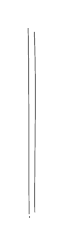
\begin{tikzpicture}[x=0.006cm,y=0.006cm]
\draw[black!55,line width=.35pt] (0,0) .. controls (2,-130) and (1,-266) .. (2,-394);
\draw[black!55,line width=.35pt] (13,-8) .. controls (18,-137) and (13,-266) .. (14,-390);
\fill (3,-400) circle (1.3);
\end{tikzpicture}} Soit $Y$ une variété élémentaire d'Artin anabélienne, (sur $K$ alg. clos), $Y\hookrightarrow J_Y^1$ son plongement dans sa jacobienne généralisée, $u\in J_Y^0(k)$ et $U$ un ouvert non vide de $Y$, tels que $U+u\subset Y$. Alors $u=1$\inserted{, ou encore : l'application $x\mapsto xu$ de $U$ dans $Y$ est l'identité.}

Par dévissage, on est ramené au cas où $Y$ est une courbe. Supposons la d'abord complète, de sorte que $U+u\subset Y$ implique $Y+u\subset Y$ -- alors le résultat est bien connu Cet résulte p.ex. de la formule des p\textsuperscript{ts} fixes, qui implique que $\tau_u\mid Y$, \inserted{si ce n'est l'identité,} a $2-2g$ p\textsuperscript{ts} fixes, ce qui (comme $g\geq2$ à cause de l'hypothèse anabélienne) est absurde.

Cela \deleted{\unsure{signifie}} \inserted{implique} donc, dans le cas général, \inserted{au moins si $g\neq1$,} que l'image de $u$ dans la partie abélienne de $J_Y^0(k)$ est nulle.

\margin{Si $g\geq2$, quitte à remplacer $Y$ par $\widehat Y$, OPS. $Y$ complète. Si $g=1$ ou 0, cf argument homologique plus bas}
\margin{ne sert à rien ici}

\deleted{[[Or d'après la structure connue de $J_Y^0$ comme extension de $J_{\widehat Y}^0$ par un tore $\mathbb G_m^I/\mathbb G_m$ (où $I=\widehat Y\unsure{\setminus|-}Y$) $u$ s'identifie à un élément de $(\mathbb G_m^I/\mathbb G_m)_{\unsure{0}}(k)$, donc est défini par $(\lambda_i)_{i\in I}$, les $\lambda_i\in k^*$, qui servent à construire un fibré inversible}
\margin{36}

\scanpage{38}
\deleted{sur la courbe ``pincée'' $Y'\deleted{\unsure{=\widehat Y\amalg_I|=\widehat Y/I}}$ (déduite de $\widehat Y$ en contractant $I$ en un pt) en identifiant les fibres \inserted{réduites sur les $y_i\in I$} du faisceau inv. trivial sur $\widehat Y$, \deleted{\unsure{en un}} à $k$ par les $\lambda_i$ -- donc entre elles. Alors $u+x$ (pour $x\in Y$) \inserted{de $J_Y^{\unsure{1|0}}$} est représenté par le faisceau $\underline O_{\widehat Y}[x]$ (associé au diviseur $x$), muni de ces $\overline m$s identifications.]}

Pour \inserted{que $x+u$} \deleted{qu'il} soit de la forme $y$ $(y\in Y)$ il faut déjà que $u+x$ et $y$ aient $\overline m$ image dans $J_{\widehat Y}^1$, ce \unsure{que|qui} \deleted{(pour un genre $g\geq1$)} \inserted{et comme l'image de $u$ dans $J_{\widehat Y}^0$ est nulle,} implique déjà \inserted{(pour un $g\geq1$)} $x=y$, donc $u=0$. Si $g\unsure{=|-}0$, donc $\nu=\operatorname{card}I\geq3$ à cause de l'hyp. anabélienne, on \deleted{\unsure{remplace}} prend une partie \inserted{$J$\unsure{,}} de $I$ à deux élts, et on remplace $\widehat Y$ par $\widehat Y\setminus J$ pour conclure encore à $x=y$ donc $u=0$.

\margin{\unsure{Cependant|Comment}, on ne sait pas que l'image de $u$ dans $J_{\widehat Y\setminus J}^0$ est nulle!}

[En fait, on a prouvé que si $u\in\operatorname{Ker}(J_Y^0-J_{\widehat Y}^0)$, alors $(Y+u)\cap Y=\unsure{\varnothing|\phi}$ -- et par ailleurs, s'il existe un ouvert non vide $U$ de $Y$ tel que $U+u\subset Y$, alors $u$ est dans le Ker précédent \unsure{(du m|celui-ci} $\neq1$). Mais ces arguments ne marchent que pour \uline{$g\neq1$}.]
\margin{$g\geq2$?}

Il vaut mieux, dans le cas général, présenter les choses sous forme \deleted{\unsure{co}}homologique. Considérons les deux \deleted{applications} \inserted{morphismes} $U\overset{i}{\lhook\joinrel\longrightarrow}Y$, inclusion
\margin{37}

\scanpage{39}
\mspage{19}
et $j:U-Y$ induit par $\tau_u$, je dis que $H_1(i)=H_1(j)$, ou ce qui revient au $=$, puisque $Y\xrightarrow{\alpha}J_Y^1$ induit un iso. $H_1(\alpha):H_1(Y)-H_1(J_Y^1)$, que $\unsure{H_1(\alpha)|H'_1(\alpha)|H_1^*(\alpha)}\unsure{H_1(i)|H'_1(i)}=H_1(\alpha)H_1(j)$, ou encore $H_1(\alpha i)=H_1(\alpha j)$.

Or on a $\alpha j=\tau_u(\alpha i)$ donc \deleted{il suffit de}
\[
H_1(\alpha j)=H_1(\tau_u)H_1(\alpha i)
\]
et on sait que $H_1(\tau_u)=\operatorname{id}$, OK. Cela étant, soit $I=\widehat Y\setminus Y$, $J=\widehat Y\setminus U$, de telle façon que $J\supset I$, \unsure{et|\deleted{et}} Soit $f:\widehat Y\simeq\widehat Y$ déduit de $j:U\subset Y$ en passant aux complétés, donc \inserted{$f(U)=\widehat Y-f(J)\subset Y=\widehat Y-I$} \deleted{\unsure{on a} $\unsure{f(J))|f(J)}$} implique $f(J)\supset I$ i.e. $J\supset f^{-1}(I)$.

On voit que le passage de $H_1(U)$ à $\unsure{H^1(Y)|H_1(Y)|H'(Y)}$, par bouchage de trous en $J\setminus I$, a pour noyau la \inserted{somme des} $L_j$ avec $j\in J\setminus I$, et pour la raison analogue le noyau de $H_1(U)\unsure{-|\to}H_1(Y)$ induit par $j$ est la somme des $L_j$ avec $j\in J\setminus f(I)$, d'ailleurs les $L_j$ $(j\in J)$ dans $H_1(U)$ sont $\simeq\widehat{\mathbb Z}$ (resp. $\widehat{\mathbb Z}'$ en car. $p>0$\unsure{..|...}) et le sous-$\widehat{\mathbb Z}$-module engendré est $\widehat{\mathbb Z}^{J}/\widehat{\mathbb Z}$ (diagonale), donc \deleted{si $\operatorname{card}J\geq3$\unsure{,}} les sous-modules engendrés par deux parties \inserted{$I,I'$} de $J$ distinctes de $J$, ne peuvent être égaux que si $I=I'$, ou $I$ et $I'$ de cardinal $\mu-1$ (où $\mu=\operatorname{card}J$)
\inserted{Mais ici quitte à rapetisser $U$, on peut supposer}
\margin{38}

\scanpage{40}
\inserted{que $\operatorname{card}I<\operatorname{card}J-1$ i.e. $\operatorname{card}(J\setminus I)=\operatorname{card}(Y\setminus U)>1$,}
\deleted{On est donc dans l'un des cas \unsure{suivts|suivants}}

\deleted{a) $f^{-1}(I)=I$ i.e. $I$ stable par $f$.}

\deleted{b)} Donc on voit que l'on doit avoir $f^{-1}(I)=I$ i.e. $I$ stable par $f$, ce qui montre que $\tau_u$ induit en fait un \uline{automorphisme} de $Y$.
\margin{\inserted{Remplaçant} \deleted{\unsure{On a donc}}}

\deleted{que $Y$ est une courbe elliptique}

dans ces arguments $Y=\widehat Y\setminus I$ par $Y'=Y\cup i=\widehat Y\setminus I'$ $(I'=I-\{i\})$, on voit de $=$ que $f$ induit un autom de $Y'$ (cet argument marche dès que $Y'$ s'injecte dans sa jacobienne généralisée, ce qui \deleted{sauf le cas où $Y$ \unsure{est} de type $(0,\nu)$ \unsure{avec}} \inserted{est le cas grâce à l'hyp. anabélienne sur $Y$)}

\deleted{\unsure{et|soit}} donc $f$ induit l'identité sur $I$. Si le genre est $0$, on en conclut (puisque $\nu\geq3$) que $f$ est l'identité; \deleted{Reste le} Dans le cas du genre $1$, on en conclut maintenant que l'image de $u$ dans $J_{\widehat Y}^0$ est égale à $1$, et on termine comme précédemment.

Ouf!
\margin{39}

\scanpage{41}
\mspage{20}
2. La question de pleine fidélité.

Soient $K,K'$ deux extensions de type fini de $\mathbb Q$ --- est-il vrai que tout $\Pi_{\mathbb Q}$-homomorphisme $\Pi_K-\Pi_{K'}$ provient d'un homomorphisme de corps $K'\longrightarrow K$? On est ramené aussitôt au cas où --- une clôture algébrique $\overline{\mathbb Q}$ de $\mathbb Q$ étant choisie, d'où un $\Gamma_{\overline{\mathbb Q}/\mathbb Q}$ --- $K$ et $K'$ ont des sous-corps $k,k'$ (clôture alg. de $\mathbb Q$ dans $K$ resp. $K'$) isomorphes, avec des \deleted{iso} \inserted{plongt} $k,\deleted{k'}\longrightarrow\mathbb Q$ de $=$ image, d'où que \unsure{$\mathcal E_K$.|$\mathcal E_{K'}$} et $\mathcal E_{K'}$ peuvent être \unsure{considérés|considérées} comme des extensions d'un même groupe $\Gamma=\Gamma_{\overline{\mathbb Q}/k}$ par $\pi_K$ resp. $\pi_{K'}$. La question est alors si \uline{tout} hom. de $\pi_{K'}$ dans $\pi_K$, qui commute à l'action de $\Gamma$, est induit par un hom $K\hookrightarrow K'$. Pour construire ce dernier, il faudrait donc avoir une idée comment reconstruire $K,K'$ à partir des extensions $\mathcal E_K,\mathcal E_{K'}$, ou encore à partir
\margin{40}

\scanpage{42}
des groupes \inserted{profinis} extérieurs avec opérations de $\Gamma$ dessus. Et on pressent que le th. 3 du \S\ précédent (appliqué notamment à $\mathbb P_K^1$ convenablement troué...) pourrait donner la clef d'une telle construction.

Bien \deleted{\unsure{en|sur}} sûr, des homomorphismes extérieurs quelconques $\unsure{\pi_{\overline{K'}}|\pi^{\wedge}_{K'}|\pi_{\widehat K'}}\longrightarrow\unsure{\pi_{\overline K}|\pi^{\wedge}_K|\pi^{\wedge}_{\overline K}|\pi_{\widehat K}}$ n'auront pas de sens géométrique --- l'idée est que les opérations du groupe $\Gamma=\Gamma_{\overline{\mathbb Q}/k}$ dessus sont si draconiennes, qu'il n'est possible de trouver un hom extérieur qui y commute que par voie géométrique --- par des plongements de corps. Donc il est essentiel ici que le corps de base ne soit pas quelconque, mais un corps tel que $\mathbb Q$ (ou, ce qui revient manifeste-ment au $=$, une extension de type fini de $\mathbb Q$). Encore faut-il se borner aux hom $\pi_{K'}-\pi_K$ dont on décrète d'avance que l'image soit ouverte --- sinon
\margin{41}

\scanpage{43}
\mspage{21}
prenant pour $\pi_{K'}$ le groupe unité (i.e $K'=k$), on trouverait un hom $K\longrightarrow k$ correspondant!

Il faut pour le moins, pour travailler à l'aise à partir d'homomorphismes $\pi_{K'}-\pi_K$ (au lieu de $\mathcal E_{K'}-\mathcal E_K$) supposer que le centralisateur dans $\pi_K$ de l'image de \unsure{tt|$\forall$} sous-groupe ouvert de $\pi_{K'}$ soit réduit à $(1)$ --- on dira que l'homomorphisme en question est \uline{anabélien}\unsure{,|.} disons --- de telle façon qu'à partir de cet hom (commutant à $\Gamma$) on reconsti-tue l'hom d'extensions $\mathcal E_K$ et $\mathcal E_{K'}$, qui est l'objet vraiment essentiel. P. ex. si justement $K'=k$, donc $\mathcal E_{K'}=\Gamma$, ce que nous intéresse, ce ne sont pas les $\Gamma$-hom de $\pi_{K'}=(1)$ (!) dans $\pi_K$, mais bien les \uline{sections} de $\mathcal E_K$ sur $\Gamma$.

\uline{Question}-\uline{conjecture} Soient $K,K'$ deux corps, extensions \inserted{de type} \unsure{finies|finie} de $\mathbb Q$, \deleted{considérons} \inserted{et} un morphisme $B_{K'}\longrightarrow B_K$ de topos sur $B_{\mathbb Q}$.
\margin{42}

\scanpage{45}
\mspage{22}
ceci est sans doute faux (cf plus bas \inserted{n\textsuperscript{o} 3}) --- il faudrait \inserted{\unsure{en}} \deleted{\unsure{donc|dans}} \inserted{renforcer} c) ci-dessus en

c') L'hom $\mathcal E_{K'}^\circ-\mathcal E_K$ induit par $\mathcal E_{K'}-\mathcal E_K$ est anabélien (où $\mathcal E_{K'}^\circ$ est le noyau de l'hom composé
\[
\mathcal E_{K'}^{\unsure{\circ}}\longrightarrow\Gamma_{\overline{\mathbb Q}/\mathbb Q}\xrightarrow{\substack{\chi\ \text{caractère}\\\text{cyclotomique}}}\widehat{\mathbb Z}^{*}).
\]

Mais pour voir que cette condition est \uline{nécessaire} pour que l'hom soit géométrique, il faudrait \deleted{\unsure{savoir}} vérifier que \inserted{pour} tout sous-groupe ouvert $\mathcal E'$ d'un $\mathcal E_K$, le centralisateur dans $\mathcal E_K$ (non seulement de $\mathcal E'$ lui-$=$, mais même de $\mathcal E'^\circ$) est réduit à $1$ --- ce qui résulte de la démonstration du th. 1, et du fait\textsuperscript{*} que pour \unsure{$\forall$|tt|$A$} sous-groupe ouvert $\Gamma'$ de $\Gamma=\Gamma_{\mathbb Q}$, le centralisateur (non seulement de $\Gamma'$, mais $=$) de $\Gamma'^\circ$ dans $\Gamma$ est réduit à $(1)$.
\margin{* à vérifier!}

Donc, la conjecture initiale \unsure{revue|ainsi} et corrigée donne la

\uline{Conséquence} (conjecturale) Pour toute \deleted{\inserted{\unsure{groupe de}}} section de $\mathcal E_K$ sur \deleted{$\Gamma_{\mathbb Q}$, \unsure{soit \illegible{1}|qui est|qui définit}} \inserted{un sous-groupe ouvert $\Gamma'$ de $\Gamma_{\mathbb Q}$,} de sorte que $\Gamma'$ opère (effectivement) sur $\pi_K$, on a \inserted{(\unsure{si} $K$ pas alg. sur $\mathbb Q$ i.e. $\pi_K\ne(1)$)} $\pi_K^{\Gamma'^\circ}\ne(1)$.
\margin{44}

\scanpage{46}
À vrai dire, à certains égards les $\Gamma_K$ sont des groupes trop gros pour pouvoir travailler directement avec, il y a lieu de regarder $\Gamma_K$ comme un $\varprojlim$ de groupes $\Gamma_{U/\mathbb Q}$ associés à des modèles affines de $K$ --- et on s'intéressera plus particulièrement à des modèles affines qui sont des variétés élémentaires --- plus généralement, qui sont des $K(\pi,1)$ (au sens profini...). Il est possible qu'il faille d'ailleurs, dans l'énoncé de la conjecture de départ, prendre un hom \inserted{ext} $\mathcal E_{K'}\longrightarrow\mathcal E_K$ dont on suppose d'avance (en plus de l'hyp. \unsure{anabélienne|anabélien} et de la compatibilité avec les hom \unsure{dans|des} $\Gamma_{\mathbb Q}$) qu'elle est compatible avec les \uline{filtrations} de ces groupes, associées à ces modèles (``\unsure{filtrations|filtration} \unsure{modéliques|modélique}'' (\unsure{grossières|grossière})).

Nous allons alors, en $=$ temps que des extensions de t.f. de $\mathbb Q$, les hom entre tels, et
\margin{45}

\scanpage{47}
\mspage{23}
homomorphismes de groupes profinis associés, \deleted{regarder} \inserted{étudier} la situation analogue pour des ``modèles'' élémentaires \inserted{anabéliens}, voire des modèles $K(\pi,1)$ généraux. (On peut aussi regarder \unsure{de|des} tels modèles sur un corps \deleted{\unsure{de nombres}} \inserted{$K$ ext.} de type fini de $\mathbb Q$ -- mais passons pour le moment sur cette situation mixte, un peu bâtarde\ldots) Si $U,V$ sont des tels modèles, tout morphisme $\unsure{V|U}-U$ définit un morphisme de topos galoisiens sur $B_{\mathbb Q}$, $B_U\longrightarrow B_V$, \deleted{\unsure{de tels|dont le|dans le}} et si $\unsure{V|U}$ est \deleted{anabélien} élémentaire anabélien, cet \unsure{homph} est connu quand on connait seulement
\[
H_1(B_{\bar U},\mathbb Z_{\ell})-H_{\unsure{1|n}}(B_{\bar V},\mathbb Z_{\ell})
\]
-- ce qui est beaucoup moins que la classe d'iso. du hom. de $B_{\mathbb Q}$-topos. (En fait, \deleted{il \unsure{suffit}} \inserted{sans hyp} anabélienne sur $V$, dès que $V$ \unsure{se|est} plonge dans une VA, $f$ est connu quand on connait son action sur les types étales\ldots). Mais quels sont les hom $B_U-B_V$, ou $\mathcal E_U-\mathcal E_V$
\margin{46}

\scanpage{48}
qui correspondent à des morphismes de modèles ? Avec un peu de culot, on dirait

\uline{Conjecture fondamentale} : Soient $U,V$ deux schémas de t.f. sur $\mathbb{Q}$, \inserted{$V$ \deleted{\unsure{séparés}} séparé} réguliers, $U$ une \deleted{\unsure{modèle}} \inserted{variété} élémentaire anabélienne sur une extension finie de $\mathbb{Q}$. \deleted{Alors} \inserted{Considérons} \deleted{tout hom} \inserted{un hom} $B_V-B_U$ des \unsure{topos|types} \unsure{étales|étale} sur $\mathbb{Q}$ -- ou ce qui revient au même, un hom de groupes extérieur
\[
f:\mathcal E_V=\pi_1(V)-\mathcal E_U=\pi_1(U),
\]
compatible avec les hom\inserted{ ext} dans $\Gamma_{\mathbb{Q}}=\pi_1(\mathbb{Q})$.
\margin{\uline{NB} pr l'instant \unsure{on se bornera surtout|on se ramènera} au cas où $V$ lui-$=$ est un modèle élémentaire anabélien, disons \unsure{dim. $1$.|donc}}

Conditions équivalentes

 a) Cet hom provient (à isom près) d'un \unsure{homomorphisme} $V-U$ sur les modèles (qui est donc uniquement déterminé)

 b) $f\mid\mathcal E_V^\circ$ est anabélien, i.e. l'image \unsure{pr|par} $f$ de $\unsure{\forall|A}$ sous-groupe ouvert de $\unsure{\mathcal E|B}_V^\circ$ a un centralisateur réduit à $1$
\margin{47}

\scanpage{49}
\mspage{24}
Pour la nécessité de b), on est ramené aussitôt au cas où $\unsure{V|U}$ est réduit à un pt, où cela se réduit à la \deleted{``\unsure{conséquence conjecturale}'' de la \unsure{conjecture-question} préliminaire.}

\margin{\figure{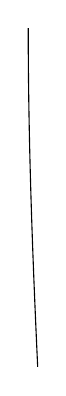
\begin{tikzpicture}\draw[thin] (0,0) .. controls (0,-1.5) and (0.06,-3) .. (0.12,-4.3);\end{tikzpicture}}}
\uline{Conséquence conjecturale} Soit $\Gamma'\subset\operatorname{Im}(\mathcal E_U\longrightarrow\Gamma_{\mathbb{Q}}\unsure{)}$ un sous-groupe ouvert, correspondant à un corps $k$ fini sur $\mathbb{Q}$, considérons un $k$-point de $U$, d'où un relèvement $\Gamma'\unsure{-|\longrightarrow}\mathcal E_U$, de sorte que $\Gamma'$ opère sur $\unsure{\Pi|\pi}_{\unsure{U|K}}$. Ceci posé\unsure{,} on a
\[
\unsure{\Pi|\pi}_U^{\Gamma'^\circ}=\{1\}.
\]

On étudiera par la suite les relations entre cette \unsure{``}\inserted{cons.} conjecturale'', et la précédente (d'apparence opposée !) concernant les $\mathcal E_K$.

La conjecture fondamentale, sur les modèles implique la conjecture fondamentale sur les corps, à condition de prendre soin, dans cette dernière, de se limiter aux hom compatibles aux filtrations modéliques,
\margin{et il vaut mieux se borner à l'\unsure{équivt.|équiv.} de a) et b) -- \unsure{la|les} \unsure{condition|conditions} c) sur les centralisateurs \unsure{risquent|risque} de passer mal à la $\varprojlim$}

Plus généralement, prenant \inserted{\unsure{complets|complètes|compacts} pour $U$} des schémas, \deleted{\unsure{de dim}} qui sont des $\varprojlim$ de \deleted{\unsure{schémas}} \inserted{modèles élém.} \unsure{anabéliques|anabéliens}, avec morphismes de transition \inserted{des imm ouvertes} affines
\margin{48}

\scanpage{50}
(pour pouvoir passer à la $\varprojlim$ dans la catégorie des schémas), pour $V$ un schéma $\varprojlim$ de schémas séparés réguliers de t.f sur $\mathbb{Q}$ (morphismes de transition \inserted{imm. ouvertes} affines sans plus), Alors les morphismes \uline{dominants} de schémas $V\longrightarrow U$ doivent correspondre aux hom ext $\mathcal{E}_V\longrightarrow\mathcal{E}_U$, compatibles avec les projections dans $\mathcal{E}_{\mathbb{Q}}\unsure{\simeq|=|\xrightarrow{\sim}}\Gamma_{\mathbb{Q}}$, et telles que l'image soit ouverte. P.ex. on pourrait prendre \inserted{pour} $U$, \deleted{$\operatorname{Spec}(\unsure{\mathcal{O}}_{X,\unsure{x}})$}\unsure{,} $V=$ les spectres d'anneaux locaux\inserted{ réguliers} \unsure{ess.|ets.|en.} de type fini sur $\mathbb{Q}$.

\figure{\begin{tikzpicture}\draw (0,0)--(.55,.03);\end{tikzpicture}}

Cette conjecture fondamentale (éventuellement revue et corrigée en cours de route !) étant admise, la question qui se pose ensuite est de déterminer les topos (pro) galoisiens sur $B_{\mathbb{Q}}$ qui proviennent de modèles élémentaires anabéliens -- ou encore, les $\unsure{\Pi_U|\pi_U}=\pi_1(\bar U)$ de tels modèles étant connus, de déterminer quelles sont
\margin{49}

\scanpage{51}
\mspage{25}
actions extérieures possibles \unsure{des|de} sous-groupes\inserted{ ouverts} $\Gamma$ de $\Gamma_{\mathbb{Q}}$ sur de tels groupes fondamen-taux -- et éventuellement question analogue pour d'autres types de groupes profinis, correspondant à des $K(\Pi,1)$ qui se réaliseraient par des variétés algébriques (sur $\mathbb{C}$, disons), mais pas par des variétés élémentaires. (J'ai en vue surtout des \deleted{topos} \inserted{variétés} modulaires, tels que, notamment, des variétés modulaires pour des courbes algébriques\ldots) À partir de là, \unsure{$\leftarrow$|on} \unsure{reconstruirait|reconstruira} par recollement, en termes profinis, tous les schémas lisses sur un corps de type fini sur $\mathbb{Q}$ (ou plutôt, la catégorie de ceux-là\ldots), ou plus gén. sur un corps quelconque -- puis, sans doute, par ``recollement'', la catégorie des schémas loc de type fini sur \unsure{$q$|\deleted{d}|\deleted{f}|$\forall$} un $K$ -- tout \unsure{au|du} moins la cat. des fractions qui s'en déduit en \deleted{\unsure{égale|égalant}} rendant inv. les
\margin{50}

\scanpage{52}
homéomorphismes universels\ldots

Les réflexions précédentes suggèrent aussi des énoncés comme \unsure{les|le} \unsure{suivants|suivant} : Pour un schém. de base $S$ loc. noeth. donné,
\margin{$S$ de car. $0$ ?}
le foncteur $X\unsure{-|\longrightarrow}X_{\mathrm{et}}$, allant de la catégorie des schémas\inserted{ réduits} loc. de prés. finie \inserted{\deleted{réduits}} sur $S$, vers la 2-catégorie des topos au dessus de $X_{\mathrm{et}}$, est \deleted{pleinement} 1-fidèle (deux hom $f,g:X=Y$ tels que les homomorphismes de topos \unsure{\inserted{$f_{\mathrm{et}},g_{\mathrm{et}}$}} $X_{\mathrm{et}}\rightrightarrows Y_{\mathrm{et}}$ au-dessus de $S_{\mathrm{et}}$ soient \unsure{ég|$fg$|\deleted{ég}|\deleted{$fg$}} isomorphes, sont égaux) et $=$ peut-être \uline{pleinement} \uline{fidèle}, quand on passe à la catégorie des fractions, de $(\mathrm{Sch}_{\mathrm{l.t.f}})/S$ obtenue en rendant inv. les homéom. universels\ldots \unsure{Exprimant|Expérimenter} \deleted{\unsure{p}} ceci p.ex. pour les autom d'une courbe alg. propre sur une ext. finie de $\mathbb{Q}$, \unsure{en|on} \inserted{re}\unsure{trouverait|trouvant|trouvait} le ``fait'' que tout autom ext. de $\mathcal E_K$ ($K$ le corps des fonctions de $X$) qui respecte la structure à lacets et qui commute à l'action de $\Gamma$, provient d'un autom de $X$
\margin{51}

\scanpage{53}
\mspage{26}
3. \uline{Étude des sections de} $\mathcal{E}_U$ \uline{sur} $\Gamma$.

Soit $U$ un \deleted{modèle élémentaire sur} \inserted{schéma connexe lisse de t.f. \inserted{\unsure{géom. conn|géom. conn.|géom. connexe|géométriquem.}}} le corps $K$, d'où $\mathcal{E}_U-\mathcal{E}_K$, et on se propose d'étudier les sections mod $\unsure{\Pi_{U/K}|\pi_{U/K}}$-conjugaison --- plus généralement, on veut en $=$ temps regarder les sections $\mathcal{E}'_K\longrightarrow\mathcal{E}_U$, où $\mathcal{E}'_K$ est un sous-groupe ouvert de $\mathcal{E}_U$ (ce qui signifie que l'on fait une extension de base finie sur $K$). Si \inserted{$K$ de type fini sur le corps $\mathbb{Q}$ et si} $U$ se plonge dans un schéma \deleted{abélien} \inserted{ou un groupe commutatif \deleted{\unsure{algébrique}} \unsure{rigide|rigides}} l'application
\[
U(K)\longrightarrow \inserted{\text{Classes d'isomorphie}}\ \text{Sections de }B_U\text{ sur }B_K
\]
i.e. classes de $\unsure{\Pi_{U/K}|\pi_{U/K}}$-conjugaison \unsure{des|de} sections de $\unsure{B_U|\mathcal{E}_U}$ sur $\unsure{B_K|\mathcal{E}_K}$

est injective. On va examiner d'autres façons \inserted{``géométriques''} de trouver des sections.

Supposons d'abord que $U$ est une courbe algébrique, \deleted{\unsure{que je suppose de|qui je suppose de}} \inserted{qui ne soit pas de} type $(0,0)$ ou $(0,1)$ i.e. $\pi_1(\bar U)=\unsure{\Pi_{U/K}|\pi_{U/K}}\ne\{0\}$ ; Alors \unsure{on a} que pour $\unsure{\forall|A}\ i\in\widehat U\setminus\bar U$ (``pt à l'infini''), le groupe de lacets $L_i$ fournit un scindage (au moins si $i$ est $/K$ i.e fixé

\margin{On a choisi un rev. universel $\widetilde U$ de $U$ pour définir $\bar K$, et $\mathcal{E}_U,\mathcal{E}_K$, et $\mathcal{E}_U-\mathcal{E}_K$}
\margin{\diagram{\begin{tikzcd}[ampersand replacement=\&,row sep=small,column sep=small]
1\&\\
\mathcal{E}_K\arrow[u]\arrow[r,equal]\&\Gamma\\
\mathcal{E}_U\arrow[u,no head]\&\\
\unsure{\Pi_{U/K}|\pi_{U/K}}\arrow[u]\&\\
1\arrow[u]\&\\
(1)\&
\end{tikzcd}}}
\margin{52}

